%!TEX root =  main.tex


Speculative decoding (SD)~\citep{leviathan2023, ryu2024closerlook-survey,xia2024sd-survey} is a popular method used for accelerating large language model (LLM) inference. 
Instead of generating tokens sequentially with the target large model, SD uses a typically smaller and faster draft model to autoregressively draft (propose) a short sequence of tokens, which the target model then verifies in parallel.
This parallel verification allows SD to achieve higher generation throughput than conventional autoregressive decoding when most drafted tokens are accepted. 
However, the effectiveness of SD is highly sensitive to the acceptance rate of drafted tokens, as drafting introduces additional computational overhead, frequent rejections can negate its benefits and even make SD slower than standard autoregressive decoding.


Prior work has improved the verification success rate (VSR) of draft tokens through methods such as specialized drafting models~\citep{cai2024medusa,li2024eagle}, tree-based drafting~\citep{wang2025opt}, and active draft token selection~\citep{wu2025tetris}. 
While these methods increase the overall VSR, they often lengthen the drafting stage due to increased model complexity~\citep{cai2024medusa,li2024eagle} or sampling overhead~\citep{wang2025opt,wu2025tetris}.
In standard speculative decoding, drafting and verification are executed \textit{sequentially}, placing drafting directly on the critical path and fundamentally limiting achievable speedups. 
This observation motivates parallelizing the two phases: since the draft model is typically much smaller than the target model, its computation can be effectively overlapped with the target model's verification.
By parallelizing the drafting and verification stages, a smaller draft model can generate draft tokens without blocking the verification process. 
When combined with an effective drafting mechanism, parallel speculative decoding hides drafting latency and yields improved overall inference performance.


Since the verification stage inherently depends on the outputs of the drafting stage, implementing parallelism in speculative decoding is nontrivial~\citep{leviathan2023}. 
Existing methods~\citep{wang2024minions,xiao2025parallelspec,timor2025distributed} typically break this dependency at the cost of substantial additional resources, such as increased GPU or memory usage \citep{wang2024minions, timor2025distributed}, or require a dedicated training stage for the draft model \citep{xiao2025parallelspec}. 
While \citeauthor{liu2025pearl} \citeyearpar{liu2025pearl} proposes a method that parallelizes drafting and verification for a single request using pre-verify and post-verify strategies, scaling this method to batched requests (multi-request) remains challenging. 
Moreover, its performance degrades when prerequisites for post-verification are not satisfied, a limitation that becomes especially severe in batched request settings.


\begin{figure}[!ht]
    \centering
    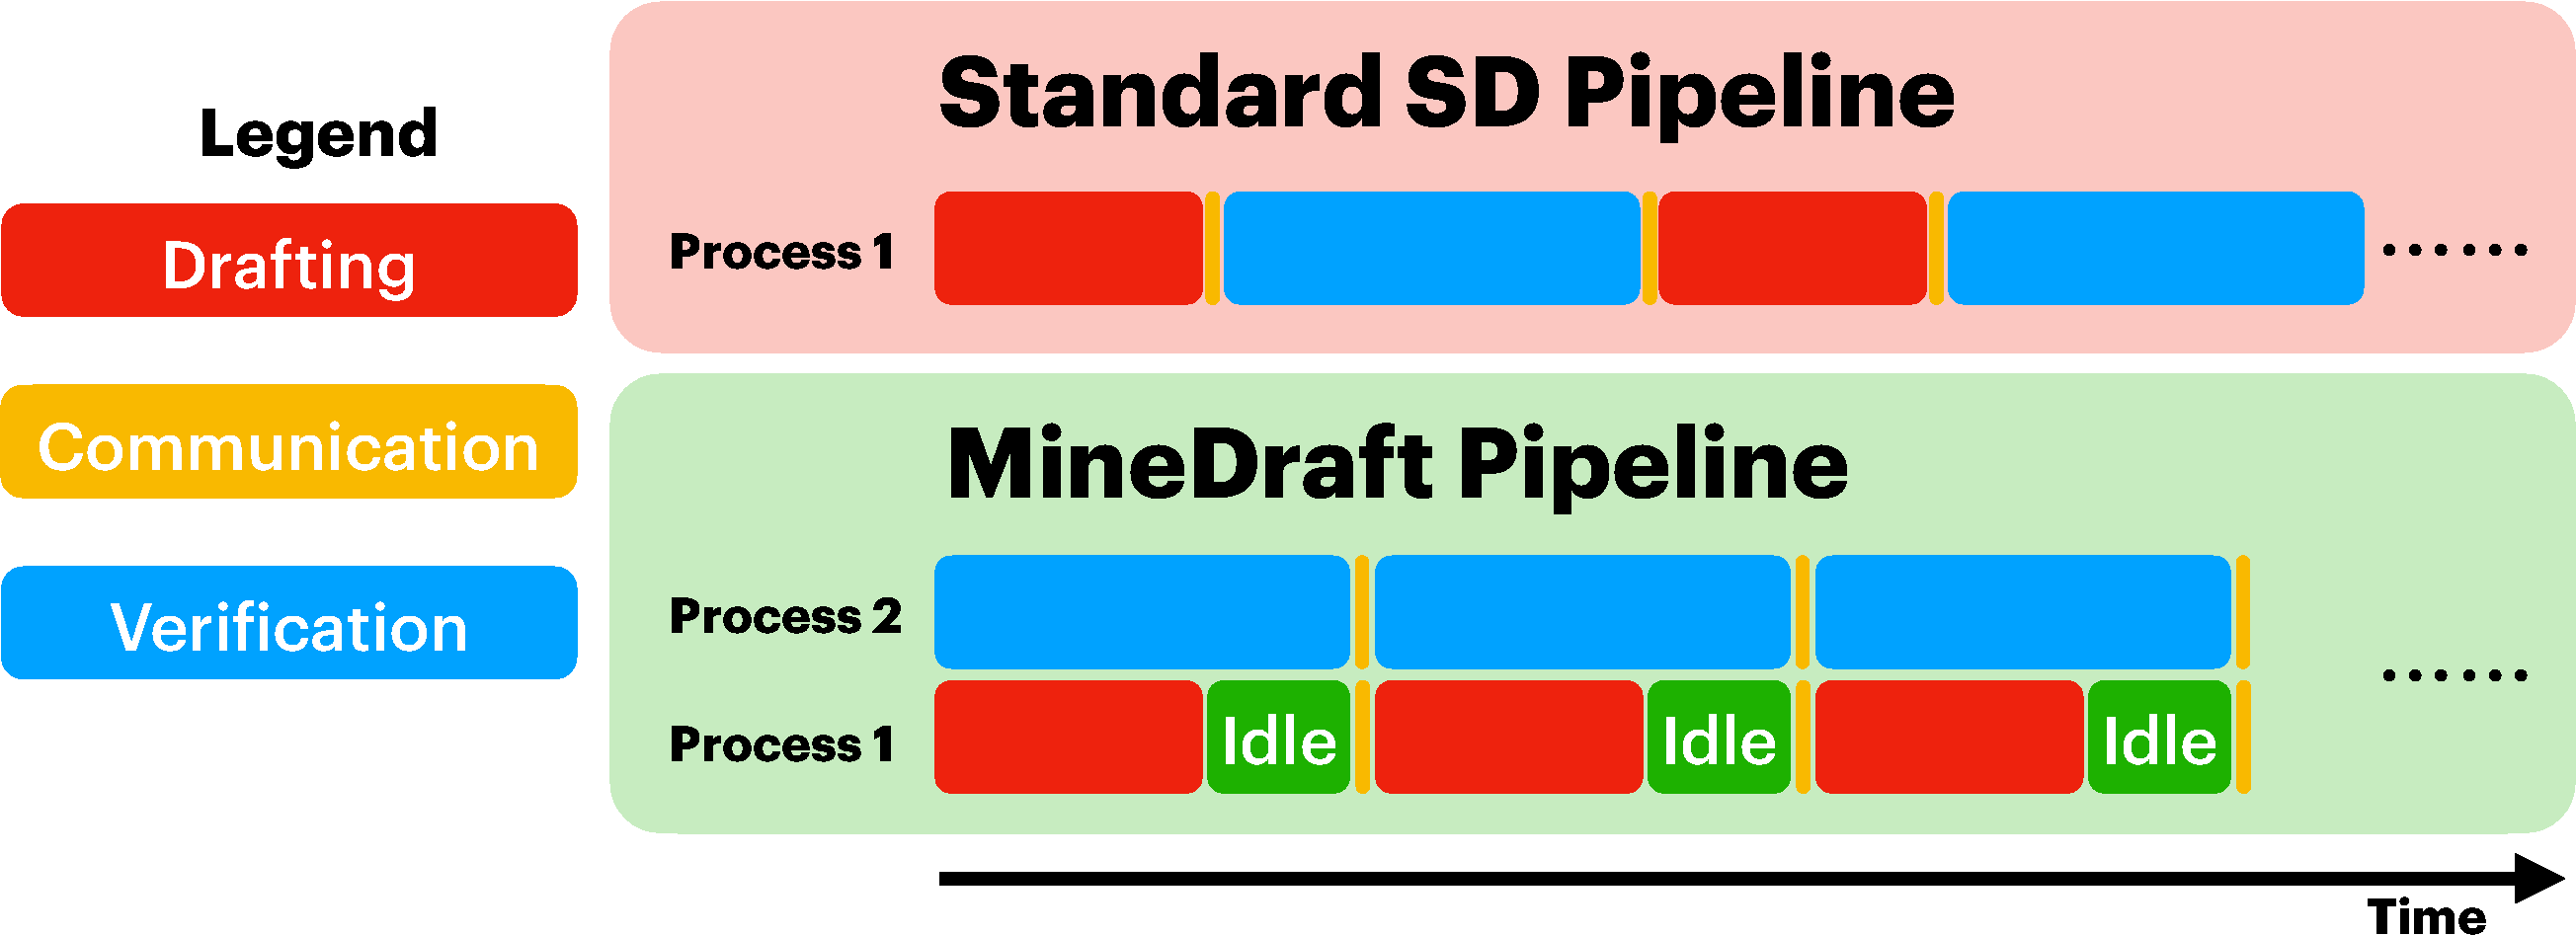
\includegraphics[width=0.96\linewidth]{figures/MineDraft-2-cropped.pdf}
    \vspace{-1mm}
    \caption{
        \textbf{MineDraft parallelizes drafting and verification:} a draft model generates tokens while the target model simultaneously verifies the previously generated draft tokens, thereby hiding drafting latency and improving overall inference throughput.
    }
    \label{fig:pipeline}
    \vspace{-4mm}
\end{figure}


This paper presents \alg{}, a framework for batch parallel speculative decoding (PSD) that systematically parallelizes the drafting and verification stages to hide drafting latency, thereby accelerating LLM inference. 
We provide a theoretical justification showing that PSD outperforms standard SD by efficiently utilizing additional computational resources through parallel drafting and verification. 
To efficiently parallelize drafting and verification, our framework uses a novel batch-parallel design that maintains two batches of requests, overlapping drafting for one batch with verification for the other.
The name of our framework is inspired by the \emph{Minecraft game engine}, which loads the next `chunk' of blocks (the next set of draft tokens) into the game world while the player is still interacting with the current blocks (verifying the current drafted tokens). This `background loading' is exactly how \alg{} hides drafting latency.


Since \alg{} is agnostic to the strategies for generating and selecting draft tokens, it can be combined with existing SD methods such as EAGLE*~\citep{li2024eagle,li2024eagle2,li2025eagle3}, PEARL~\citep{liu2025pearl}, and TETRIS~\citep{wu2025tetris}, and is orthogonal to most LLM inference optimization techniques, including forward-pass modifications, model parallelism, and draft models.
Our experimental results show that \alg{} outperforms standard SD by achieving average throughput gains and reducing end-to-end latency at the cost of only 1 additional GPU, highlighting its significant practical impact.
Furthermore, \alg{} is implemented as a plugin for the production-ready inference library vLLM~\citep{kwon2023vllm}. 
The specific contributions of this paper are summarized as follows:


\vspace{-3mm}
\begin{itemize}[leftmargin=*]
	\setlength\itemsep{-0.1em}
    \setlength{\itemindent}{2pt}
    \item \textbf{Theoretical efficiency of PSD.}
    In \cref{sec:theoretical_analysis}, we first present a theoretical analysis of batch PSD demonstrating that it achieves at least a 37\% reduction in end-to-end latency compared to standard SD under mild assumptions about the quality of the draft model.
       
    \item \textbf{A framework for batch PSD.}
    In \cref{sec:minedraft}, we propose a novel framework, \alg{}, for batch PSD that maintains two batches of requests, overlapping drafting for one batch with verification for the another. To enable parallel execution, \alg{} runs the draft model on a separate GPU and employs direct GPU-to-GPU communication to transfer draft tokens to the target model, which runs on GPUs separate from the draft model.
   
    \item \textbf{Experimental results.}
    In \cref{sec:experiments}, we evaluate the performance of \alg{} through comprehensive experiments across existing SD methods. Our results show that \alg{} achieves average throughput gains of up to $75$\% and reduces end-to-end latency by up to $39$\% compared to standard SD, at the cost of one extra GPU.

    \item \textbf{\alg{} as a vLLM plugin.}
    We develop a plug-and-play vLLM plugin that implements \alg{}, encouraging further academic research and experimentation. The plugin also supports continuous batching (iteration-level scheduling)~\citep{yu2022orca} and is fully compatible with PagedAttention~\citep{kwon2023vllm}, highlighting its significant practical impact and ease of use. The code is publicly available in the \href{https://github.com/electron-shaders/MineDraft}{MineDraft GitHub repository}. 
\end{itemize}
